\chapter{STRIPS yield mapping}

\OUTLINE{Introduce section} In this section, we illustrate the
functioning and the results of our methodology when applied to yield
monitor data collected from the same agricultural site over the
years. We start with a detailed discussion of the production of the
yield map for one specific year, and we finally show some resulting
visualizations for the same fields but different crops and years.

\OUTLINE{Introduce data context} The data arises from a study
conducted at the Neal Smith National Wildlife Refuge in central Iowa
to quantify the impact of grassland-to-cropland conversion on
nitrate-nitrogen (NO\textsubscript{3}–N) concentrations in soil and
shallow groundwater and to assess the potential for perennial filter
strips to mitigate increases in NO\textsubscript{3}–N levels, run-off
reduction, and soil nutrient loss \citep{Zhou2010}. The experiment was
run in different study sites within the 3000-ha area managed by the
U.S. National Fish and Wildlife Service, located in the Walnut Creek
watershed in Jasper County, Iowa. In this case study, we focus on one
specific site named Basswood that is situated west to the Basswood
Trailhead.

\OUTLINE{Introduce data specifics} Basswood, located at WGS84 15 N
0477097E 4598644N, has a total area of approximately 13 Ha. Nearly
81\% of the surface is cropland; most of the remaining proportion is
reconstructed prairie vegetation planted as part of the experimental
design. For the purpose of our yield maps, these areas are treated as
voids because no data were collected from that surface. Cropland in the
experiment is in a maize–soybean rotation using standard no-till soil
and weed-management techniques. Geographic coordinates, sample time,
moisture content, and maize (2008, 2010, 2012, 2014) and soybean (2009,
2011, 2013, 2015) flow rate were reported by a Case IH AFS Pro-600
combine-mounted yield monitor every 1-3 s during crop harvest,
resulting in a fine-scale spatially referenced dataset of crop yields
across the study area. \cite{Schulte2017} provides a detailed account
of the experiment protocol and the resulting improvements in the
biodiversity and the delivery of multiple ecosystem services.

\OUTLINE{Describe data} The yield monitor dataset for the year 2012
has 4,239 observations logged every three seconds starting from the
southwest corner of the site. The swath width was reported to be
constant at 6.10m. The distance traveled during each cycle, with
an overall mean of 3.7 m, has three modes with centers at 1.9, 4.0,
and 6.0 m. The distribution of the yield reported by the monitor, with
its median located at 6.3 mg/ha and the 90\% of observations being
within 1.4 and 10.8 mg/ha, is symmetric and platykurtic. Visual
inspection suggests that there are approximately 20 extreme values on
the right tail. Small areas within the field boundaries without data,
visualized as voids in the maps, correspond to small portions of soil
allocated for nonproductive purposes (e.g. perennial crops, research
equipment).

\begin{figure}[h!]  \centering
  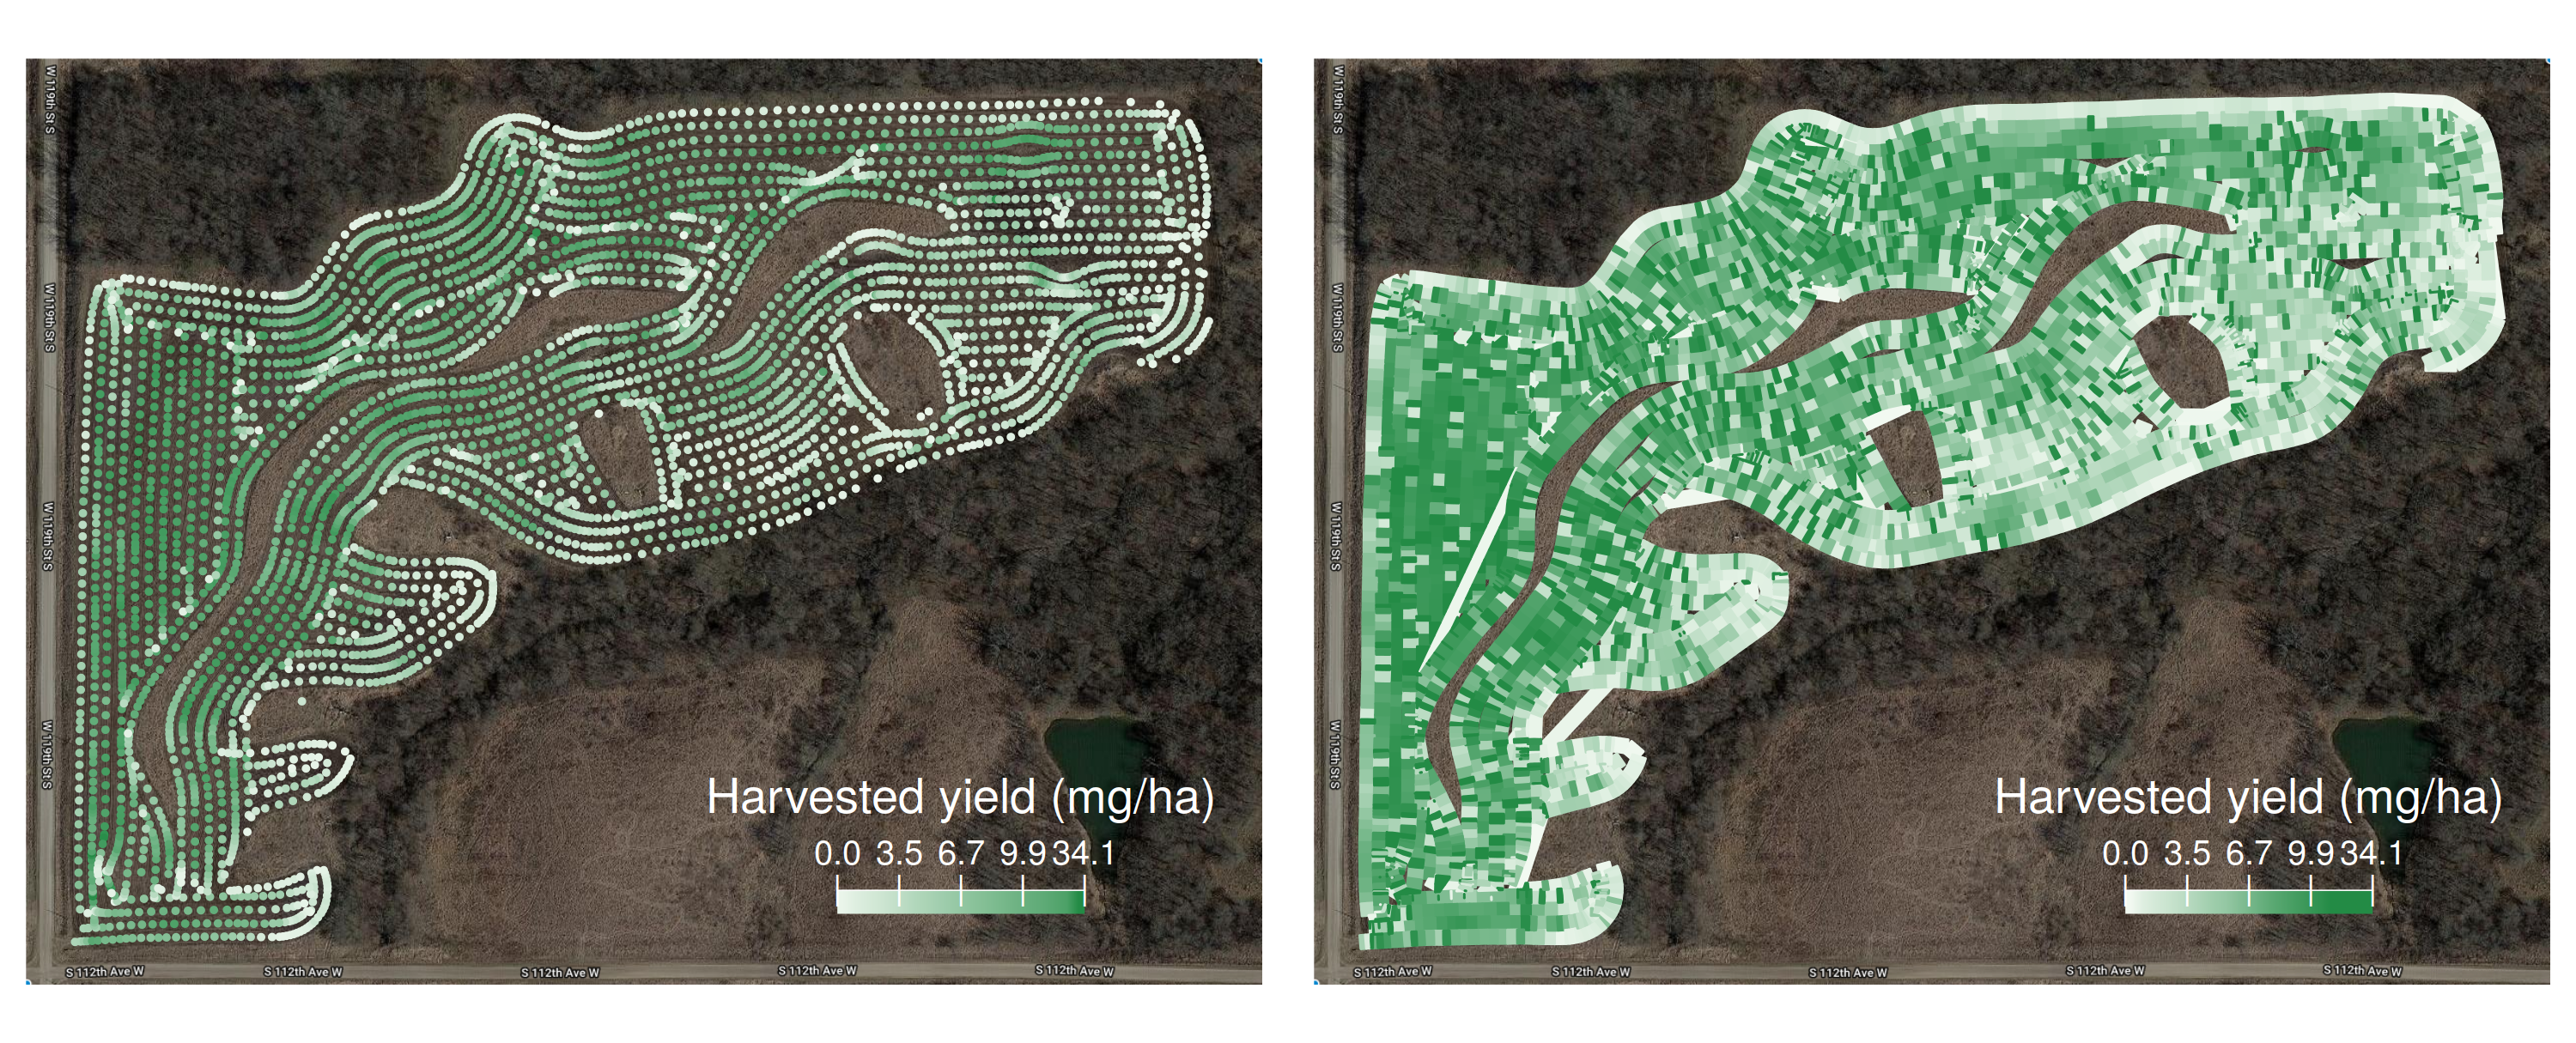
\includegraphics[width=\textwidth]{basswood_2012_res5_points_vehicle}
  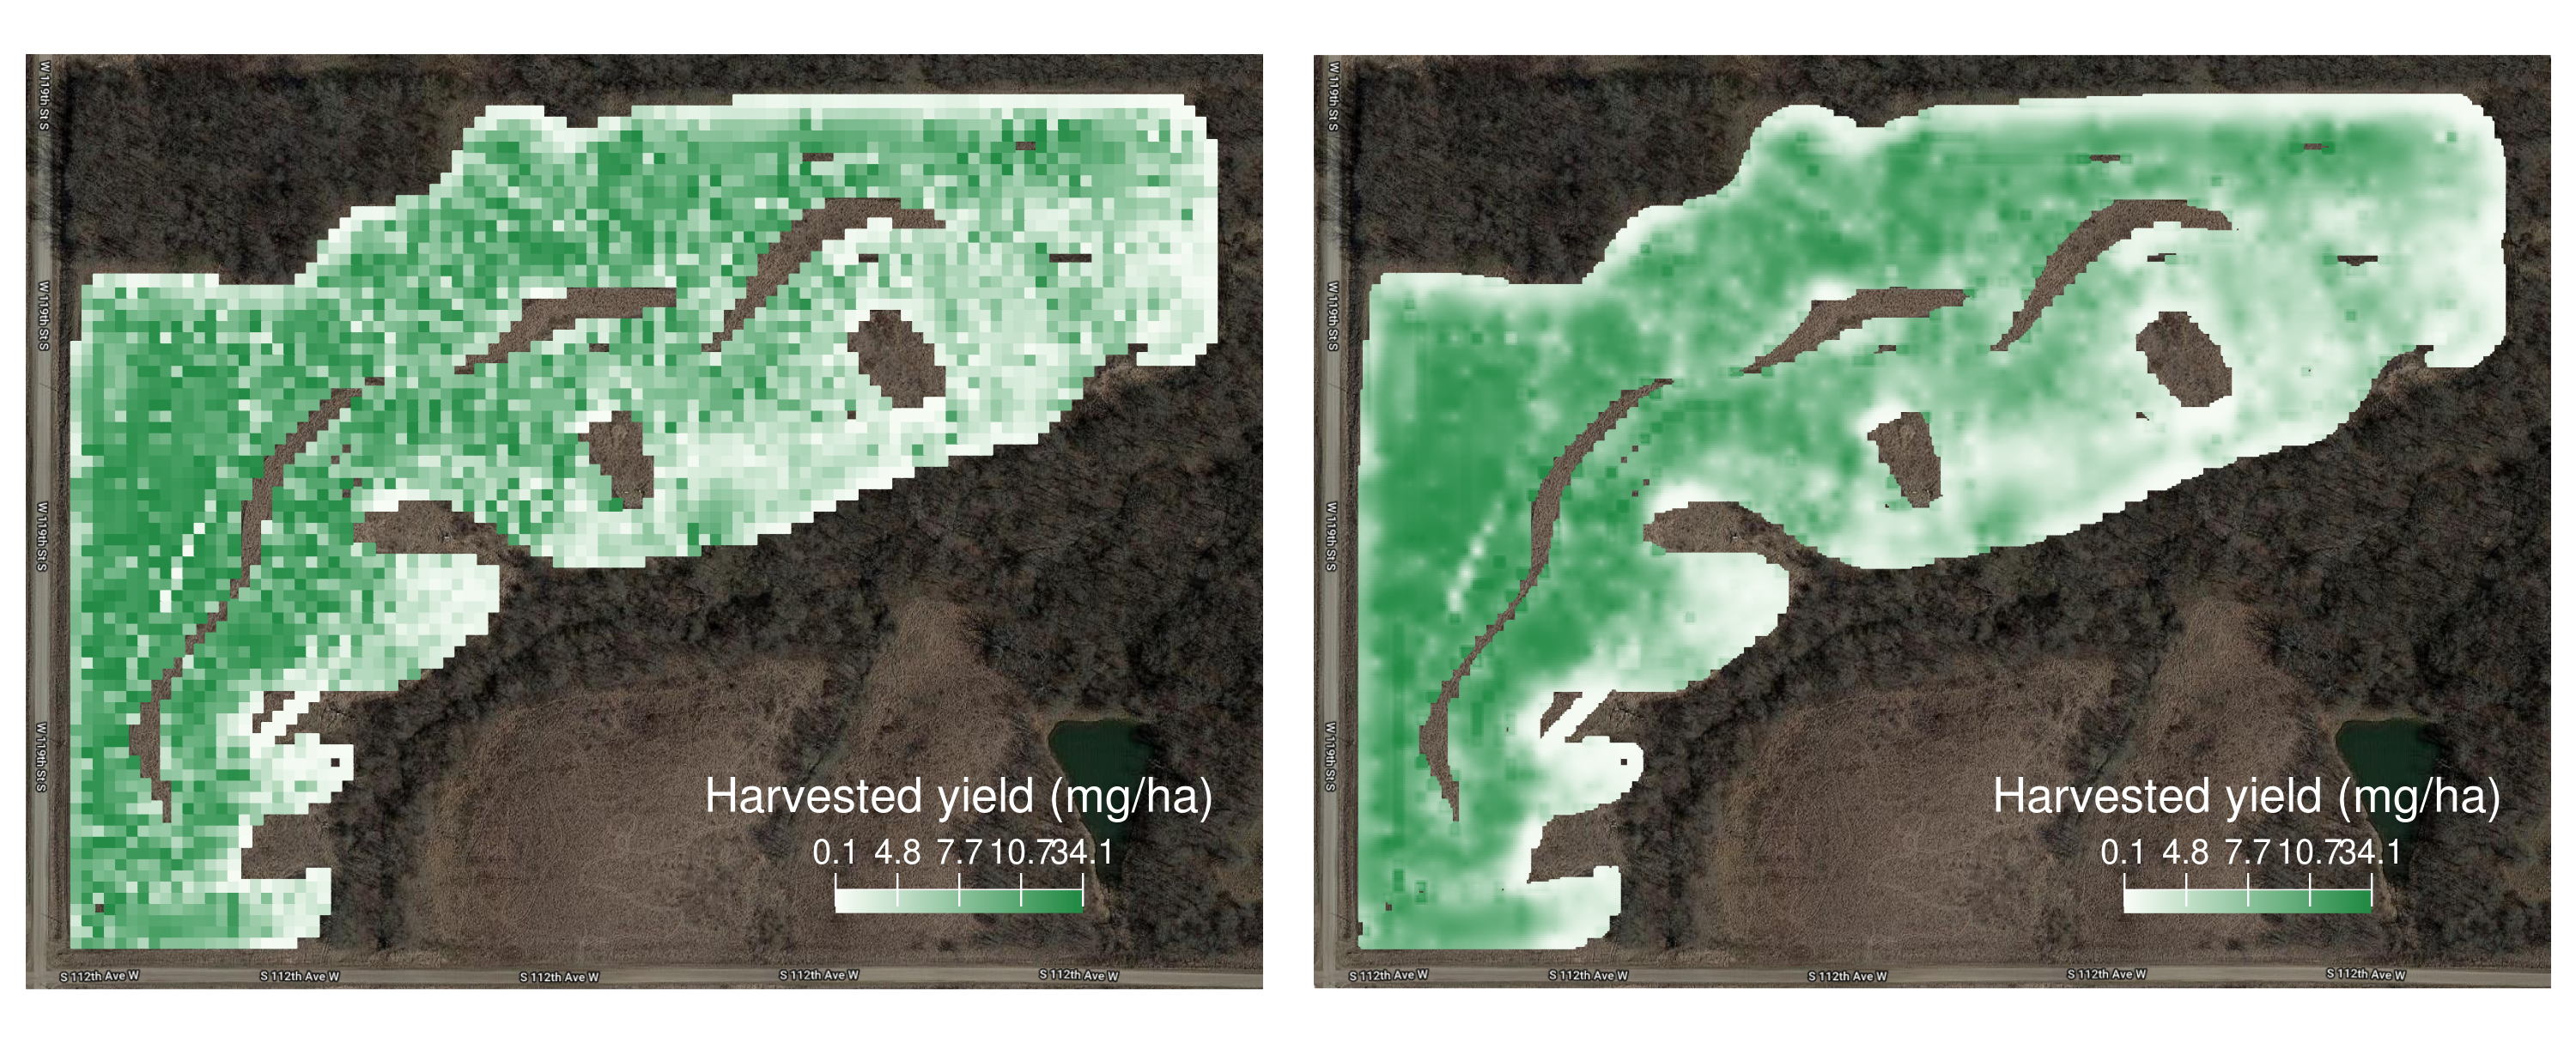
\includegraphics[width=\textwidth]{basswood_2012_res5_1_agg_smoothed}
  \caption[Visualization of selected algorithm steps as applied to a
  specific dataset]{Visualization of selected intermediate steps involved
    in the algorithm for the harvested grain yield of Basswood on year
    2012 (maize). \underline{Top left}: Point map where each observation is
    marked with equally-sized points placed at the each logging
    location. Information relevant to spatial trends are hard to observe,
    such as area coverage and overlaps. \underline{Top right}: Map of the
    clipped polygons. Highly intertiment coloring in noisy areas hinder
    the visualization of the spatial trends, hence the need for
    smoothing. \underline{Bottom left}: Map of the aggregated grid at a 5
    m resolution. This step produces equally-sized, regularly-shaped
    polygons suitable for spatial interpolation. \underline{Bottom right}:
    Map to be shown to the user. By increasing color homogeneity at a
    local level, low and high yield areas have a larger contrast and
    become easier to identify.}
  \label{fig:basswood2012-main-steps}
\end{figure}

\OUTLINE{Introduce dot maps} Figure \ref{fig:basswood2012-main-steps}
(top left) displays the simplest form of a yield map. Data points are
visualized as equally-sized symbols with colors indicating the yield
value at each recorded location. A single-hue shade of green is chosen
to ease the interpretation with dark shades being intuitively
associated with higher crop yield. The characteristics of the yield
distribution vary largely across sites, crop types, and years. Since
the main objective of yield map analysis is to identify sub-field
areas with different performance levels, the points are colored
according to a measure of relative yield within the dataset as opposed
to an absolute scale. As a general rule, we define the color gradient
as a function of the the empirical quartiles in order to guarantee
that low and high yield measurements are uniformly represented at the
same time that the interpretation guidelines remain consistent across
maps.

\OUTLINE{Describe dot map} The proposed coloring scheme helps
capturing the large-scale spatial trends: the east area, both above
and below the perennial crop strip, and the northwest area show the
best relative performance whereas the southwest area is
underperforming. Another evident pattern is outer borders and borders
around inner voids displaying lower yield, which could be explained by
soil fertility properties or could simply be a byproduct of how data
is collected. Data artifacts due to narrow finishes are well
documented: if the header cut was not full when harvesting the
boundaries and the operator failed to manually flag it, yield would be
underestimated. Careful consideration should be given to neighboring
points that are not on the borders. Light green points on the northern
borderline are adjacent to dark green points, suggesting that this
might very well be an artifact due to deficiencies in the the data
collection procedure. On the other hand, data points on the southwest
zones are consistently underperforming, thus suggesting the existence
of an actual spatial trend.

\OUTLINE{Criticize dot map} Using points to visualize the data
provides no information about the shape of the areal observational
unit and hides the overlaps in the harvested areas, which should be
considered appropriately when computing the estimated yield at a given
spatial location. In fact, from the figure it is not evident that
there is 9.0\% of areal overlap, defined as the percent excess of the
sum of the individual rectangles area over the polygons union area.

\OUTLINE{Step 1: Create polygons} We apply the RITAS algorithm. Figure
\ref{fig:basswood2012-all-steps} (top right), displaying the
constructed spatial polygons, makes overlapping patterns more evident:
(i) subsequent samples overlap during turns, especially on the inner
side; (ii) near voids, where the landscape requires more maneuvering;
(iii) wedges formed by perpendicular passing, for example on the
western part of the field; (iv) driving from one part to another; (v)
between parallel passings and narrow segments.

\OUTLINE{Step 2: Clipping} Because overlapping produces a systematic
overestimation of the effective area size, thus biasing down the
estimated yield, its correct treatment can uncover underperforming
areas. In all these cases, the coloring suggests that highly
overlapping polygons are associated with lower yields. We note,
however, that yield was computed using the theoretical polygon area
which overestimates the effective harvest area. In Figure
\ref{fig:basswood2012-all-steps} (middle left), which shows the
reshaped polygons and the yield computed with the new effective area,
we notice that some of the sub field areas with low-yield polygons now
display a better performance suggesting that this visual artifact was
indeed caused by the overlapping. As a computational note, when
producing the reshaped polygons, 10 spatial polygons whose area had
been fully harvested in previous time steps were dropped from the
dataset causing an minor leakage of 0.1\% of the total harvest mass;
in case of major situations, aggregating the mass of fully nested
geometries would be appropriate.

\OUTLINE{Motivate smoothing} As the ultimate goal of the visualization
work is to support the user's decision making process, the clipped
map is not adequate. Crop management decisions at a sub-field scale
are based on spatial trends whereas the measurements are highly noisy
due to a combination of at least 10 possible types of data collection
error as discussed in \cite{Lyle2013}. For example, in Figure
\ref{fig:basswood2012-all-steps} there are zones of predominating high
and low yield contaminated with scattered observations with the
opposite color, and there are also zones with a combination where it
is difficult to identify local trends.

\OUTLINE{Steps 3 \& 4: Gridding and tiling.} Smoothing is thus
typically applied. As discussed in the previous section,
off-the-shelf smoothing techniques are not suitable for
unequally-sized polygons. We superimpose a grid with 4,194 squares at
a 5-meter resolution and apportion the harvested mass of the reshaped
polygons into the corresponding pixels. As we retain those pixels with
at least 50\% of their area covered by observations only, we find
local zones with under or over coverage. Overall, the whole grid
covers 2.6\% less of the sampled surface, a discrepancy that can be
diminished by increasing the grid resolution.

\OUTLINE{Step 5: smoothing} The results are seen in Figure
\ref{fig:basswood2012-main-steps} (bottom right). The effect of
smoothing on the signal to noise ratio is evident from the figure. The
richness of smoothing is not only on the visualization, but also on
the interpretation of the estimated parameters. We then propose that
yield maps should not only include the spatial polygons, but also
statistical information useful for the map user. The range, for
instance, is informative for map users to better understand the scale
of the spatial effect and adjust the scale of their decisions
accordingly. % define the spatial scale of their management decisions.

\OUTLINE{Step 5: smoothing cnt'd} The smooth map is consistent with
the main spatial trends observed so far. Clear patterns become more
evident now; in the mixed areas, smoothing helps not only to identify
the overall local trend but also to make internal breaks/borders more
visible. Additional features can help with interpretation include
contour lines, e.g. \ each 1 mg/ha similar to \cite{Blackmore1999}, or
color schemes based on spatial clusters.

% Using 10 cores, the total computational time of 201 m included 168 m
% (83\%) and 17 m (8\%) spent in the smoothing and tiling steps
% respectively. This suggests that the algorithm has be run offline for
% any moderately-sized datasets, but could be improved vastly by
% simplifying the spatial interpolation model. The resulting maps for
% the same field but different years and crops are shown in Figure
% \ref{fig:basswood-history}.

\begin{figure}[h!]  \centering
  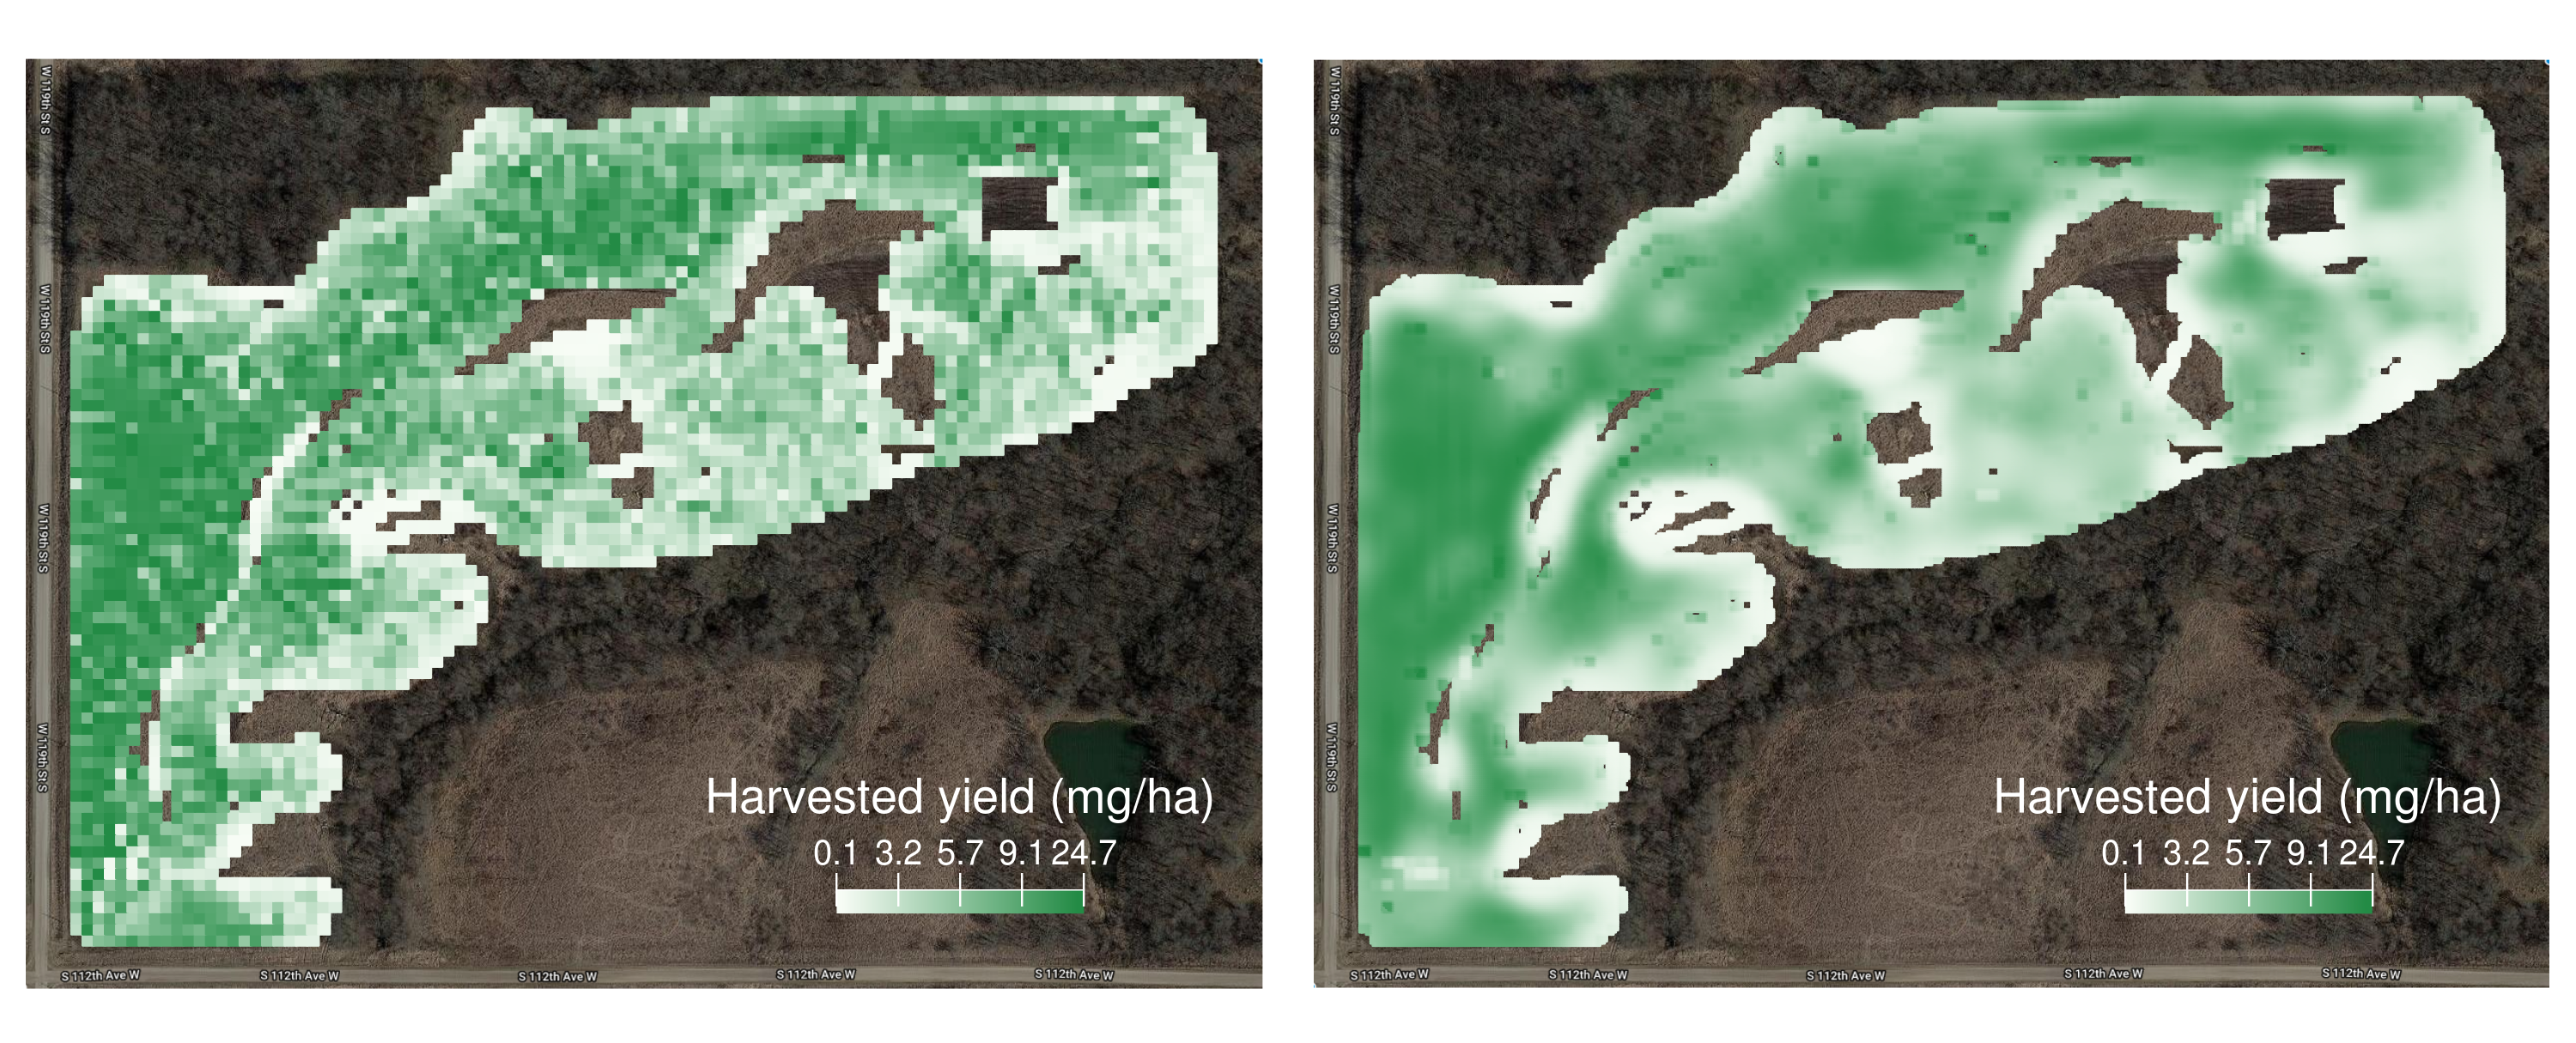
\includegraphics[width=0.49\textwidth]{basswood_2010_res5_1_agg_smoothed}
  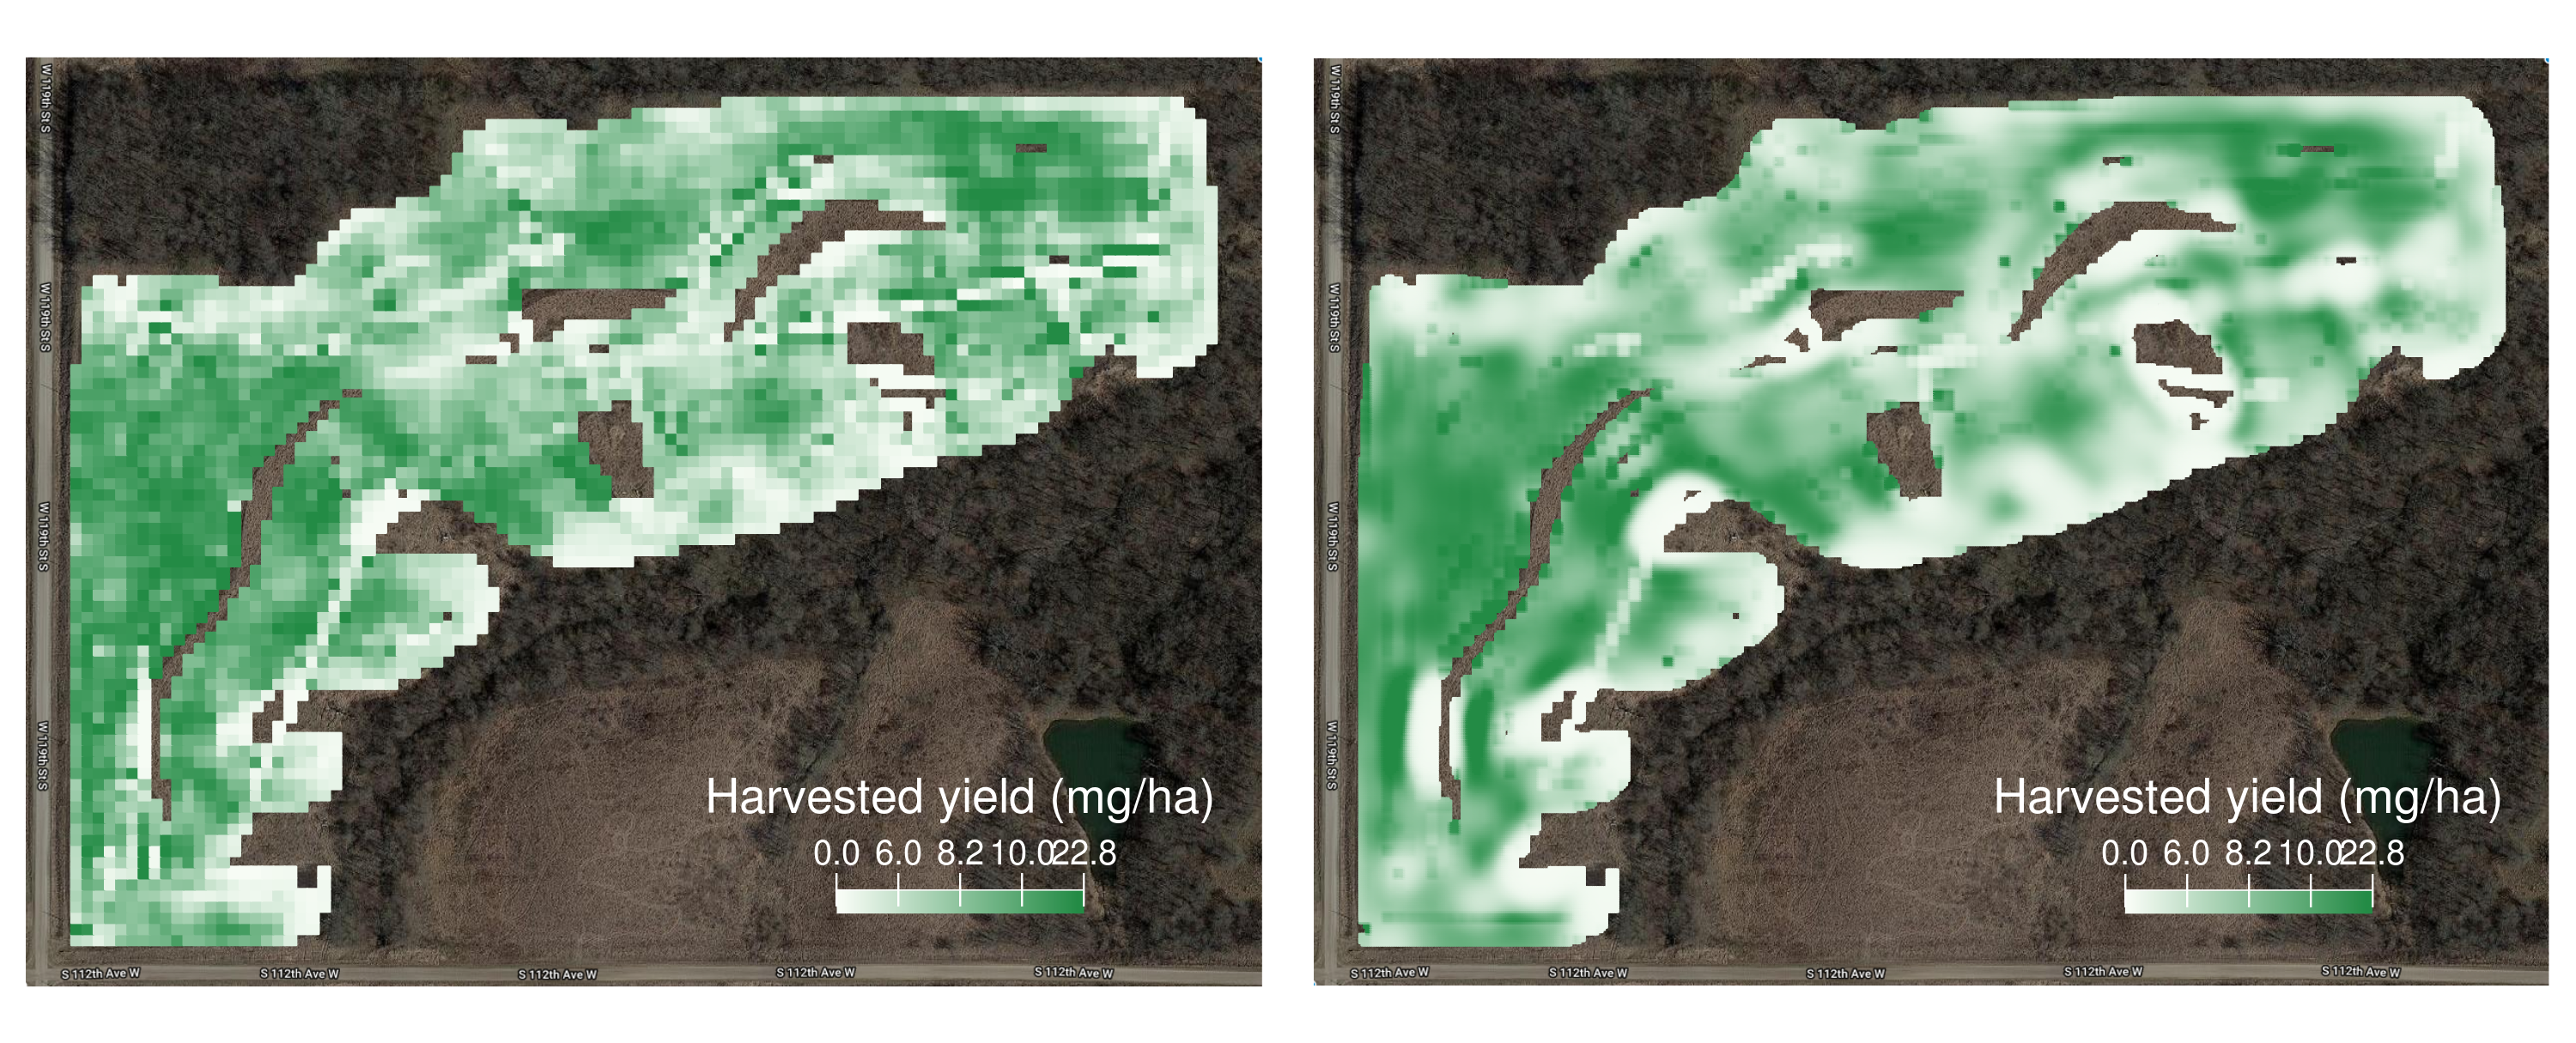
\includegraphics[width=0.49\textwidth]{basswood_2014_res5_1_agg_smoothed}
  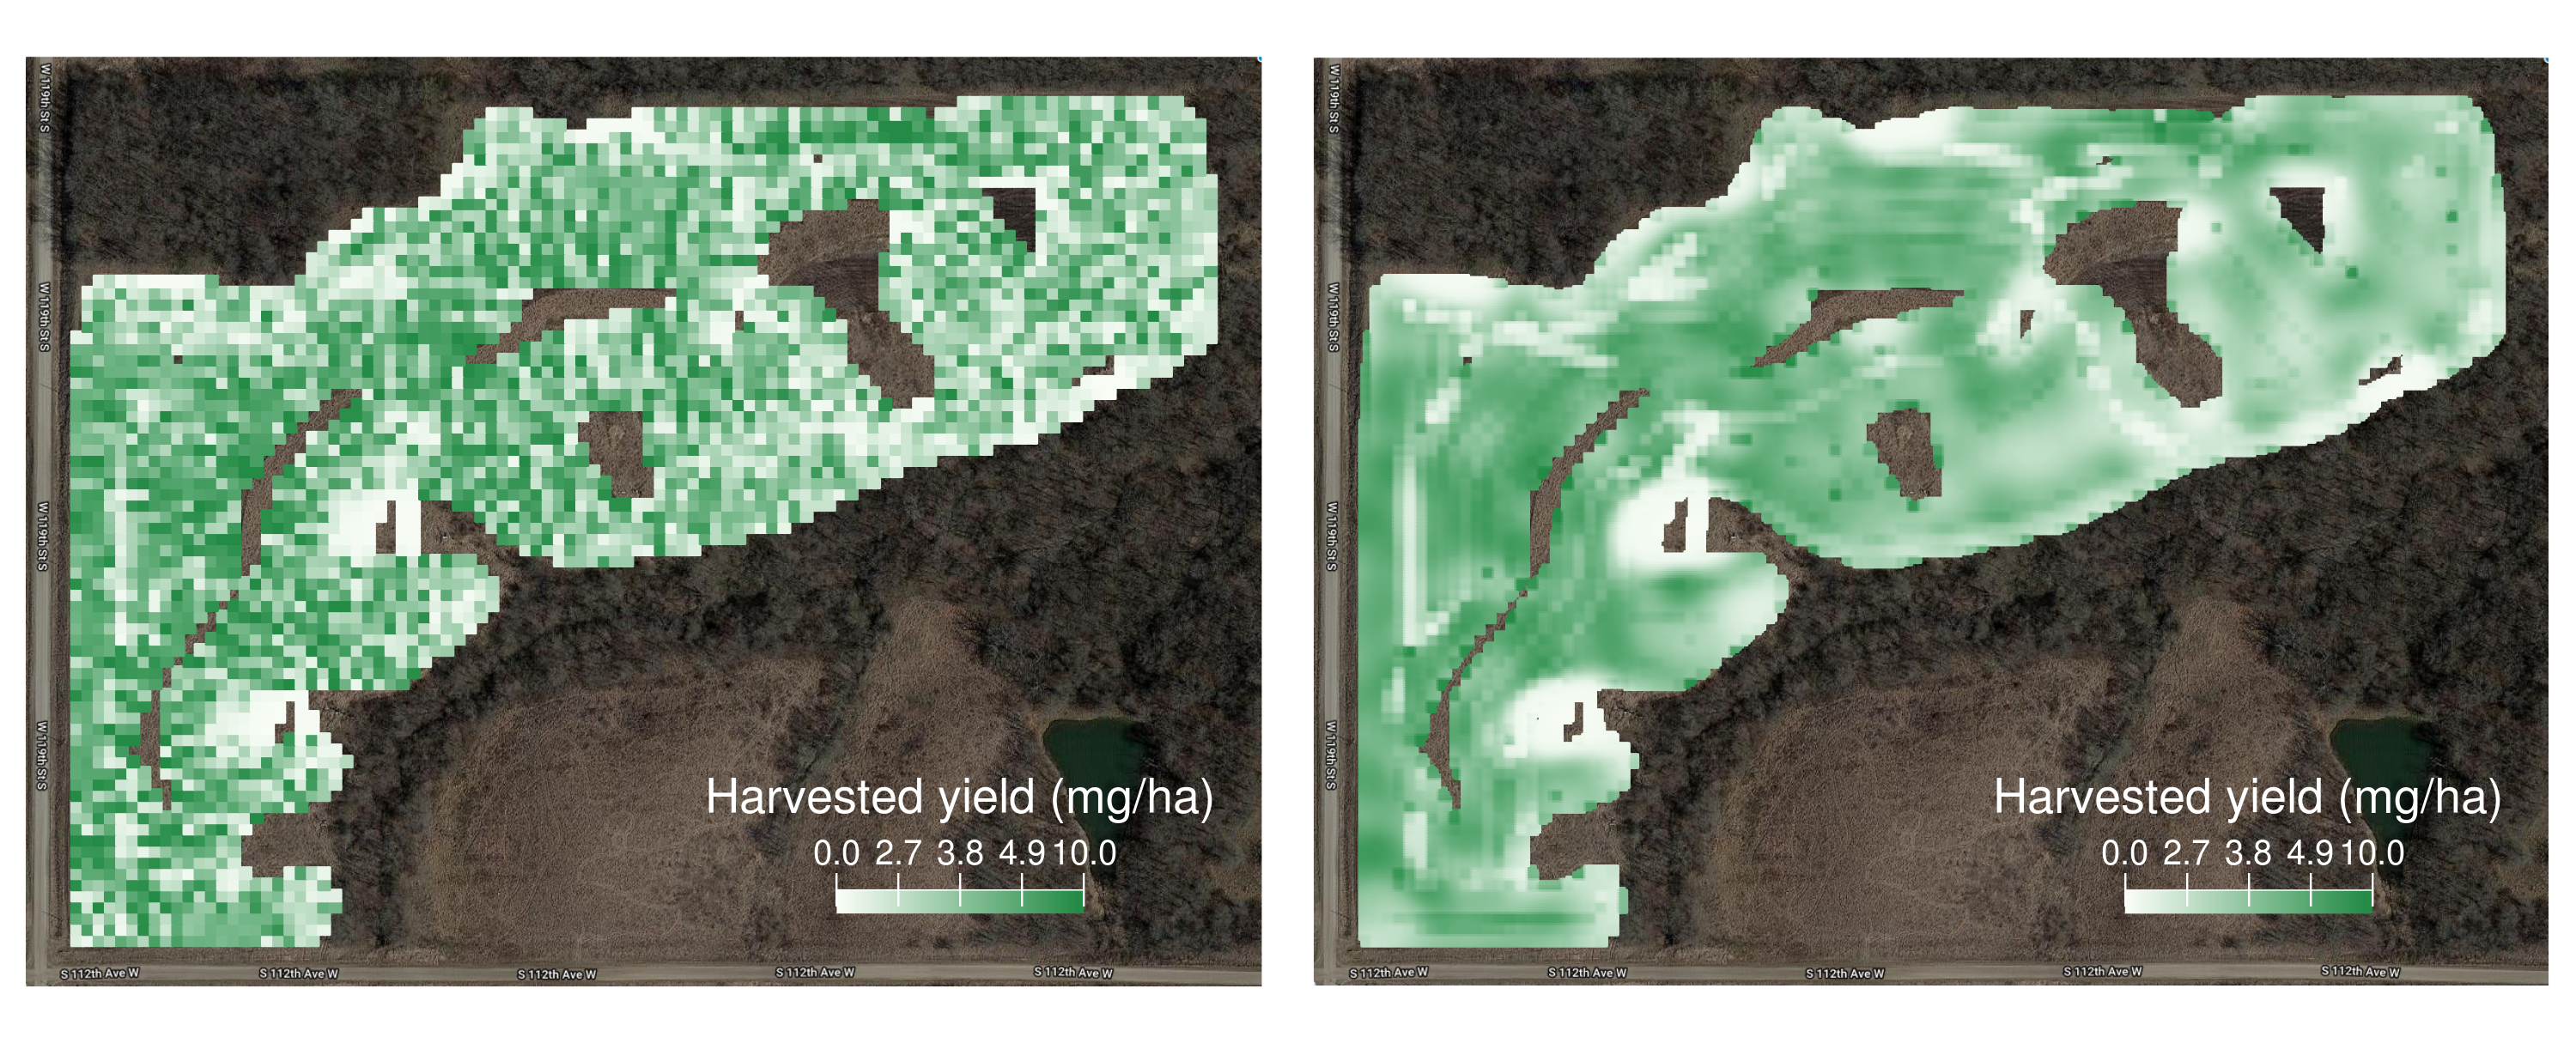
\includegraphics[width=0.49\textwidth]{basswood_2009_res5_1_agg_smoothed}
  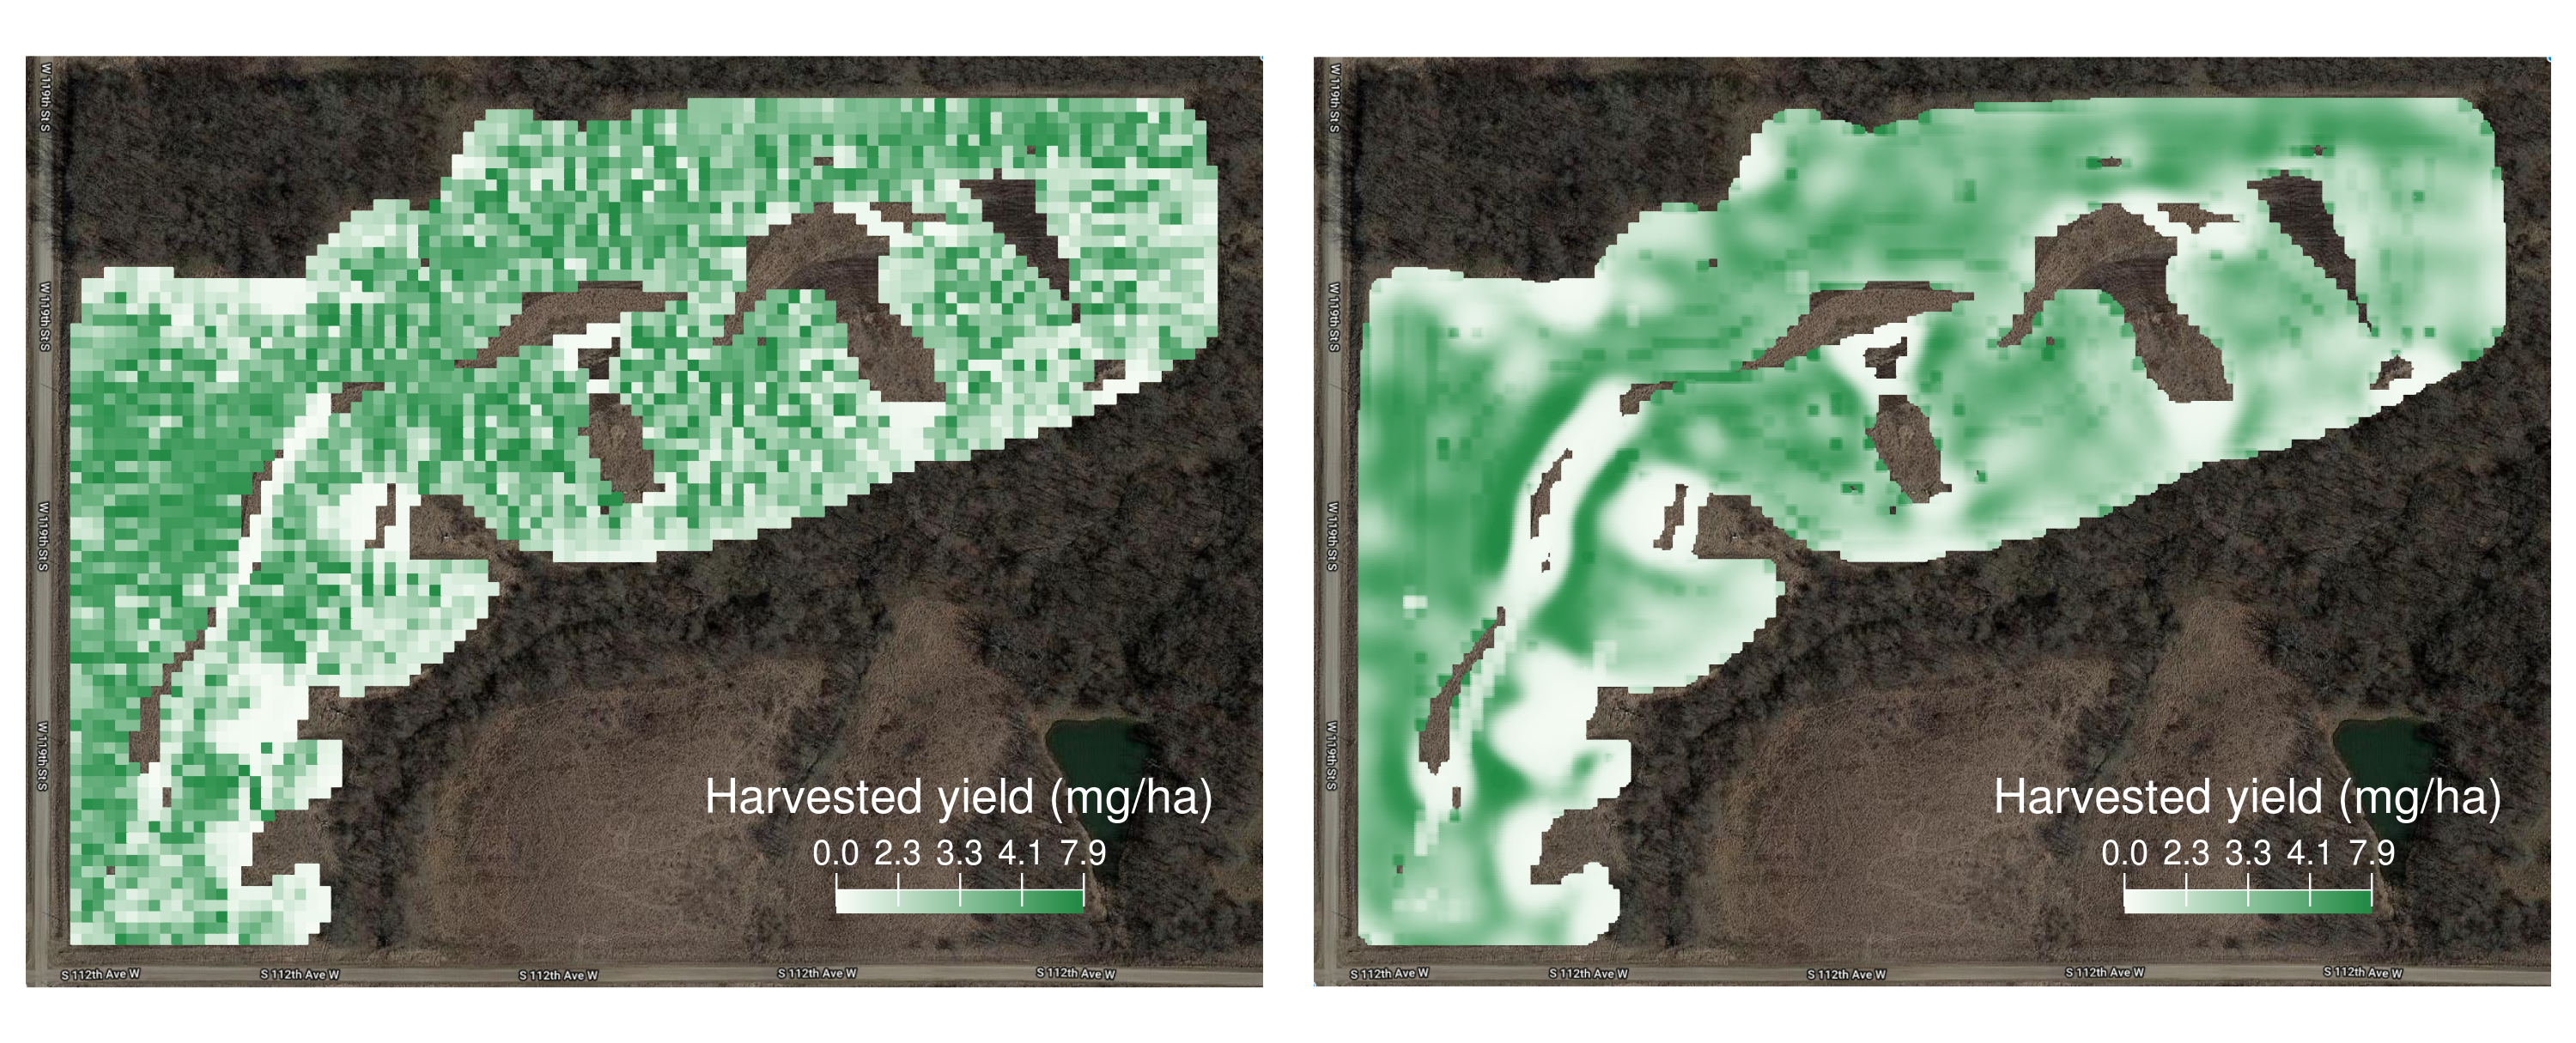
\includegraphics[width=0.49\textwidth]{basswood_2011_res5_1_agg_smoothed}
  \caption[Visualization of the algorithm output for one field across
  four different years]{Visualization of the harvested grain yield for
    Basswood in four different years. Maize in the top row, soybean in
    the bottom row. Aggregated yield in odd columns, smoothed yield in
    even columns. Although soybean data shows larger variability, as
    clearly displayed on the aggregated grid, the smooth map offer a
    clear visualization of the spatial trends. }
  \label{fig:basswood-history}
\end{figure}

%%% Local Variables:
%%% mode: latex
%%% TeX-master: "../thesis"
%%% End:
